\section{92 - MAT - WS 1.1, AN 1.2, AN 1.3, AB 1,1, FA 1.4, WS 4.1  - Bitcoin - Matura 2017/18}

\begin{langesbeispiel} \item[6] %PUNKTE DES BEISPIELS
			Bitcoin (W�hrungsk�rzel: BTC) ist eine digitale Kunstw�hrung. Der Marktwert des Bitcoin ergibt sich aufgrund von Angebot und Nachfrage.
			
Nutzer/innen des Bitcoin werden in dieser Aufgabe als Bitcoin-User bezeichnet.

Die nachstehende Abbildung zeigt den Bitcoin-Euro-Kurs vom 11. M�rz 2015 bis zum 11.�M�rz�2016. Die linke Skala zeigt dabei den absoluten Wert eines Bitcoins in Euro, die rechte Skala zeigt die Ver�nderung in Prozent bezogen auf den 11.�M�rz�2015.

\begin{center}
	\resizebox{0.8\linewidth}{!}{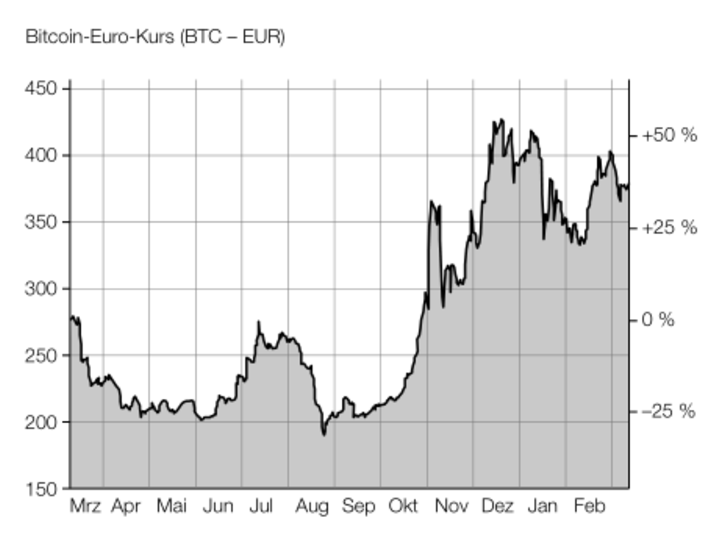
\includegraphics{../Bilder/Bild92-1.eps}}
\end{center}

\subsection{Aufgabenstellung:}
\begin{enumerate}
	\item Gib an, in welchem der Monate von April 2015 bis Dezember 2015 der Bitcoin-Euro-Kurs jeweils vom Monatsanfang bis zum Monatsende absolut am st�rksten gefallen ist, und gib diesen Kursverlust in Euro an!\leer
	
	Monat:\,\antwort[\rule{3cm}{0.3pt}]{August}\leer
	
	Kursverlust:\,\antwort[\rule{3cm}{0.3pt}]{$\approx$ \EUR{55} Toleranzintervall: $[50;70]$}
	
	Es sei $K_1$ der Bitcoin-Euro-Kurs zum Beginn des betreffenden Monats, $K_2$ der Bitcoin-Euro-Kurs am Ende des betreffenden Monats sowie $AT$ die Anzahl der Tage des betreffenden Monats.
	
	Berechne den ungef�hren Wert des Ausdrucks $\dfrac{K_2-K_1}{AT}$ und interpretiere das Ergebnis im gegebenen Kontext!
	
	\item Anfang J�nner 2016 waren ca. 15 Millionen Bitcoins im Umlauf. Die $t$ Jahre nach dem Jahr 2009 im Umlauf befindliche Menge an Bitcoins ist ann�hrend $f(t)=21\cdot 10^6-21\cdot 10^6\cdot e^{-0,18\cdot t}$. Damit ist $f(0)$ die zu Anfang J�nner 2009 im Umlauf befindliche Menge an Bitcoins.
	
	Bestimmen und interpretiere die relative (prozentuelle) �nderung der im Umlauf befindlichen Menge an Bitcoins im Zeitintervall $[7;8]$!
	
	Gib eine Gleichung an, mit der derjenige Zeitpunkt berechnet werden kann, ab dem nur mehr eine Million Bitcoins in Umlauf gebracht werden kann, und ermittle diesen Zeitpunkt!
	
	\item Eine Untersuchung der Demografie von Bitcoin-Usern hat ergeben, dass weltweit 88\,\% der Bitcoin-User m�nnlich sind.\\
Es soll festgestellt werden, wie hoch dieser Prozentsatz in �sterreich ist. Dazu wird eine gro�e Anzahl an Personen befragt. Diese Befragung ergibt, dass 171 der befragten Personen Bitcoin-User sind, und von diesen 171 Personen sind 138 m�nnlich.

\fbox{A} Gib aufgrund dieser Daten ein symmetrischen 95-\%-Konfidenzintervall f�r den unbekannten Anteil der m�nnlichen Bitcoin-User unter allen Bitcoin-Usern in �sterreich an!

Gib an, welches Konfidenzniveau zur Berechnung eines solchen Intervalls mindestens angenommen werden muss, damit der weltweit ermittelte Anteil von 88\,\% in diesem Intervall enthalten ist!

	\end{enumerate}
	
	\antwort{
\begin{enumerate}
	\item \subsection{L�sungserwartung:} 

$\dfrac{K_2-K_1}{AT}\approx -1,8$

M�gliche Interpretation:\\
Im August 2015 betrug die durchschnittliche Kurs�nderung pro Tag ca. \EUR{-1,8}.\\
oder:\\
Im August 2015 betrug der durchschnittliche Kursverlust pro Tag ca. \EUR{1,8}.

Toleranzintervall: $[-2,3;-1,5]$ bzw. $[1,5;2,3]$

\item \subsection{L�sungserwartung:} 

$\dfrac{f(8)-f(7)}{f(7)}\approx 0,065$

Toleranzintervall: $[0,06;0,07]$

M�gliche Interpretation:\\
Die Anzahl der im Umlauf befindlichen Bitcoins nimmt im Zeitraum von Anfang J�nner 2016 bis Anfang J�nner 2017 um ca. 6,5\,\% zu.\leer

M�gliche Gleichung:\\
$f(t)=20\cdot 10^6$

L�sung der Gleichung: $t\approx 17$

Ungef�hr Anfang J�nner 2026 kann nur mehr 1 Million Bitcoins in Umlauf gebracht werden.

Toleranzintervall: $[16;17]$ bzw. $[2025,2026]$
\item \subsection{L�sungserwartung:}

$n=171$, $h\approx 0,807$\\
$0,807\pm 1,96\cdot\sqrt{\frac{0,807\cdot(1-0,807)}{171}}\approx 0,807\pm 0,059 \Rightarrow [0,748;0,866]$

Toleranzintervall: unten: $[0,74;0,75]$ oben: $[0,86;0,87]$\leer

M�gliche Vorgehensweise:\\
$0,880-\frac{138}{171}\approx 0,073$

$0,073\leq z\cdot \sqrt{\frac{0,807\cdot(1-0,807)}{171}} \Rightarrow z\geq 2,418$

$2\cdot\Phi(2,418)-1\approx 0,984$

Das Konfidenzniveau muss mindestens 98,4\,\% betragen.

Toleranzintervall: $[0,98;0,99]$
\end{enumerate}}
	
	\end{langesbeispiel}